%TEX root = ../dissertation.tex

\iffalse \bibliography{bibliography/dissertation} \fi

\chapter{Designing a Programming Environment for Generative Design}
\label{chapter:pegd}

This chapter presents the design of a coherent system integrating the previously studied techniques for interactive programming tools. The first part discusses the importance of good design principles in software engineering, highlighting the lack of tools that enforce those principles in the current programming systems, specially in Architecture area where programming methods are increasingly popular among novices. The second part introduces concrete tools for documenting a program, and a framework mechanism for providing immediate feedback as the programmer write their code. While the following chapter discusses technical aspects and software architecture, this chapter focuses on conceptually build these tools and elaborates on the rationale behind all design decisions.

\section{Design Principles} 

Programming is hard to learn. Unfortunately, as shown in the previous section, few programming languages or environments are designed to introduce the basics of good software engineering practice. Specially in Architecture, the environments used to support \gls{gd} either they are old or obsolete, or they enforce particular programming methods that are inadequate, or they are not pedagogic, meaning that they are not designed for the particular programming skills of the \gls{gd} community.

The literature is vast, but it is clearly divided in two perspectives: software engineering perspective, or psychological/educational perspective. That means either systems designed for expert programmers~\citep{carlson2005eclipse,intellij2001intellij,lighttable,boudreau2002netbeans,guckenheimer2006software}, or systems designed for novices~\citep{papert1980mindstorms,goldberg1983smalltalk,GuoSIGCSE2013,Reas2006}. However, while programming systems designed for expert programmers are constantly being updated, systems designed for novices are usually obsolete or in disuse. It negatively affects other communities that are not focused on developing software for industry, but for their own purpose.

For example the \gls{gd} community is focused on build software to support Architecture methods, however designers are in desperate need of a programming system that correspond their needs. These needs are from different natures, for instance give support to the increasing adoption of \gls{gd} methods, deal with the increasing complexity of \gls{gd} programs, and above of all take into account the architect's workflow and methods helping to improve it.

In the next sections I discuss some design principles that improves in the program comprehension and also program documentation. Most of these principles were relevant contributions that, unfortunately, are vaguely represented in current systems, mainly considering the system used in \gls{gd} area. For that reason, I propose a generic implementation of a modern programming environment that meets the \gls{gd} community needs. 

\section{Program Documentation}

Program documentation is a software requirement of the utmost importance because it is a key factor for understanding programs. Even the best program, the most perfectly suitable for the job, will be essentially useless if the people who need to use it do not know what it is; cannot understand it well enough to use, build, or modify it; or (worst of all) misunderstand it and apply it incorrectly. And all of the effort, analysis, hard work, and insightful design spend to construct it will have been wasted.

Software exists for a specific reason and documentation exists to explain this reason. Every piece of code has its rational and a reason to be written in that way. Then, the documentation collects all these rationales organizing them in a form of different artifacts, such as requirements description, architectural models, data models, \gls{api} documentation, flow diagrams, use case diagrams, etc. Therefore it is, undoubtedly, a rich source of information not only for the developer who did the software, but also for the developer who will test the application, for the stakeholder who will use the application, and eventually for the developer who will maintain that code.

In fact software maintenance, traditionally defined as any modification made on a system after its delivery, is a dominant activity in software engineering. Some reports place maintenance at 90\% of the total cost of a typical software project~\citep{seacord2003modernizing,pigoski1996practical}. One of the main difficulties in software maintenance is a lack of up-to-date documentation~\citep{de2005study}. As a result, some studies indicate that 40\% to 60\% of maintenance activity is spent simply studying existing software~\citep[p. 475 and p. 35 respectively]{pigoski1996practical,pfleeger1998software}. Having an updated documentation would dramatically reduce the effort spent in this study, helping the developer to comprehend the code and maintain it.

The sad truth is that writing program documentation today is perceived as a tiresome task, if it is done at all, is often treated as an afterthought, something people do because they have to~\citep{sousa1998survey}. Bass et al. summarizes many possible reasons that lead programmers to write the documentation, and then concluded as follows:

\blockquote{Maybe a contract requires it. Maybe a customer demands it. Maybe a company's standard process calls for it. In fact, these may all be legitimate reasons. But none of them are compelling enough to produce high-quality documentation.~\citep[p. 327]{BassClementsKazman201210}}

Producing a high-quality documentation should be a natural developer's attitude not because it's ``required" but because they see that it is essential to the matter at hand. The documentation defends the developer's job because it speaks for him, for example in agile methods it can be used as a contract~\citep{ambler2007agile}. It also helps developers reason about the architecture design of their programs, and communicate these ideas while the development is in progress. However produce useful documentation is a hard task and developers have to consider that some documentation artifacts are more important than others.

As described earlier, documentation is composed by several artifacts, formally defined as any artifact intended to communicate information on the software system~\citep{forward2002relevance}. This communication is aimed at human readers, from the technical document delivered to the developer team, until the user manual delivered to the users. But the central point from where the documentation comes from is the source code, as a result it is the most important artifact as suggested in the following study:

\blockquote{Source code and comments are the most important artifact to understand a system to be maintained. Data model and requirement description were other important artifacts. Surprisingly, and contrary to what we found in the literature, architectural models and
other general view of the system are not very important. This could simply indicate that such documentation artifacts are used once to have a global understanding of the system and never consulted again after.~\citep[p. 74]{de2005study}}

The importance of source code and comments is a reality already noted in software industry, consequently the use of automation tools to generate, verify, and maintain the source code documentation, is a well known practice. The most frequently cited technologies, as concluded in~\citep{forward2002relevance}, are Javadoc\footnote{\texttt{http://docs.oracle.com/javase/7/docs/technotes/guides/javadoc/}} and DocWiz\footnote{\texttt{http://docwiz.sourceforge.net/}} to comment Java source code, Doc++\footnote{\texttt{http://docpp.sourceforge.net/}} and Doxygen\footnote{\texttt{http://www.stack.nl/dimitri/doxygen/index.html}} to comment source code in languages such as C, C++, and also Java. These tools generate an on-line documentation browser (in HTML) and/or an off-line reference manual (in $\mbox{\LaTeX}$) from a set of documented source files. The comments are inserted directly in the source code between a start tag and a end tag. Typically, these tags use the language's comment delimiter to avoid any compilation error, as a result the compiler will ignore any word between comments. Javadoc requires an extra asterisk, when compared with C standard comments (i.e. \pythoninline{/* */}). So, to generate the documentation the comments must be inside these tags (as shown in Figure~\ref{fig:javadoc-code}). Additionally, other tags are provided to document the code, for example the function parameters (\texttt{@param}), the function return (\texttt{@return}), an exception that may be thrown (\texttt{@exception}, \texttt{@throws}), and so on. As a result, these tags add proper information into the HTML page (e.g. as shown in Figure~\ref{fig:javadocgen}).

\begin{figure}[h]
\centering
\begin{subfigure}{.5\textwidth}
  \centering
  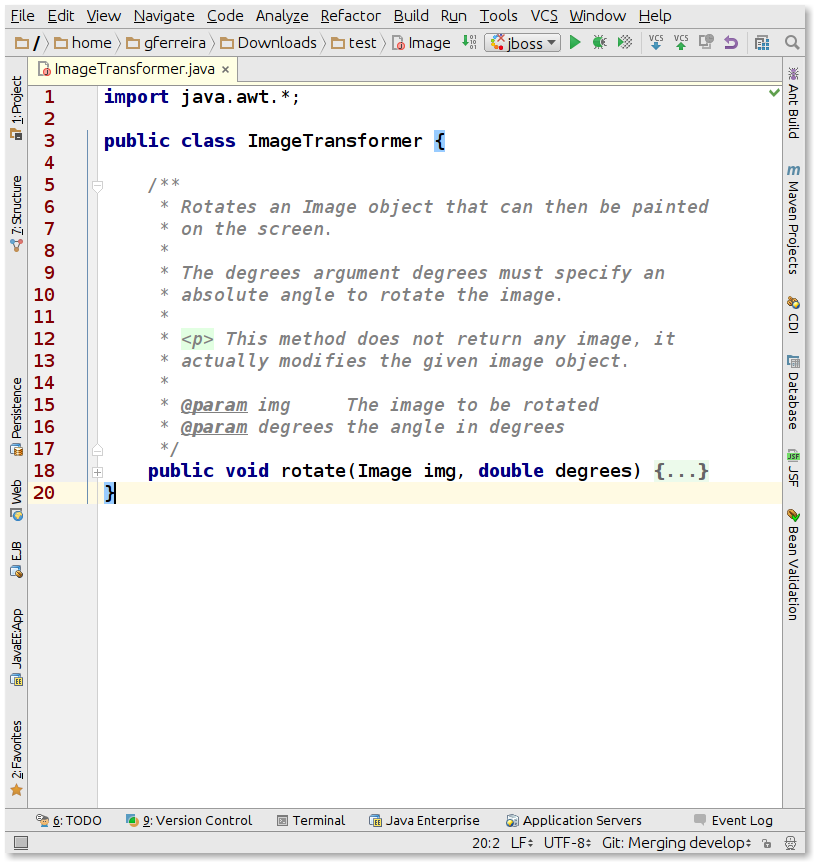
\includegraphics[width=.9\linewidth]{images/javadoc-code}
  \caption{A Javadoc annotation of a Java method}
  \label{fig:javadoc-code}
\end{subfigure}%
\begin{subfigure}{.5\textwidth}
  \centering
  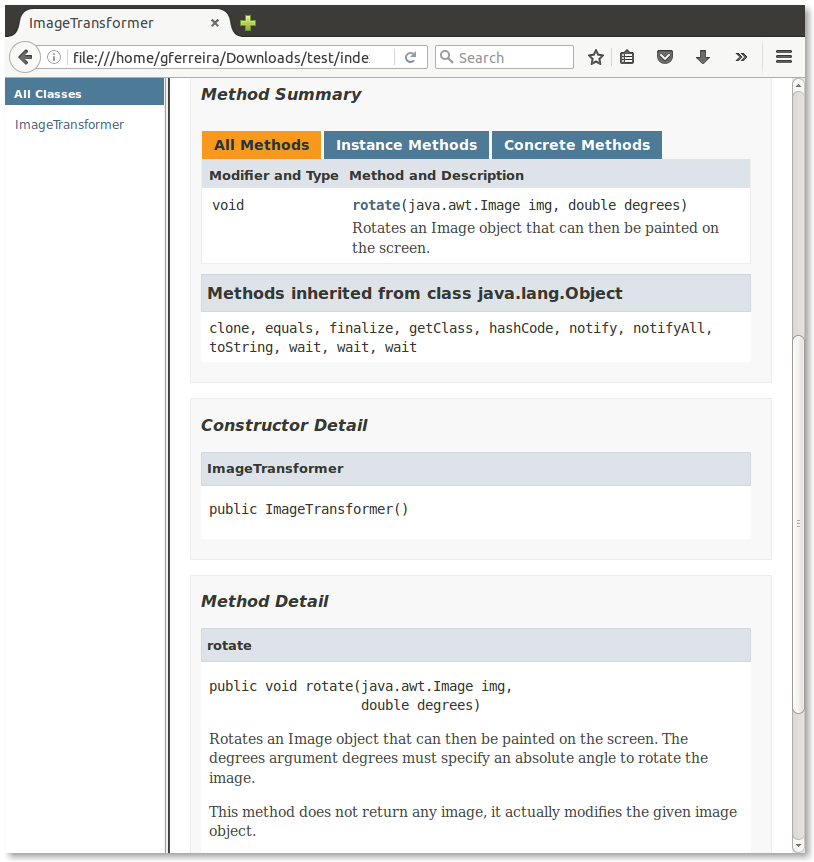
\includegraphics[width=.9\linewidth]{images/javadoc}
  \caption{Javadoc HTML auto-generated}
  \label{fig:javadocgen}
\end{subfigure}
\caption{Javadoc generation of a HTML page from a documented Java method. In the left is the source code commented with the opening tag \texttt{/**}, in the right is the generated documentation page.}
\label{fig:javadoc}
\end{figure}

Figure~\ref{fig:javadoc} shows an example of Javadoc an industry standard tool which provides interesting functionalities for documenting Java classes. The HTML format keeps information together giving the convenience of being able to hyperlink related documentation. As a result, programmers can easily navigate through classes and their respective methods. Moreover, Javadoc provides a widely integration trough \glspl{ide} (e.g. Eclipse, IntelliJ, NetBeans, etc) so programmers can generate automatic Javadoc comments using those \glspl{ide}. However these kind of tools are inadequate for other purposes.

For example, the documentation are essentially represented as rows of plain text. Despite of supporting HTML format, the generated pages only includes text and hyperlinks, media-rich resources are unsupportable. Moreover, the developer's attention is taken from code into a series of static pages which contain little information, actually they show less than the source code. And the automatic comments generated by \glspl{ide}, are useless comments that add none rigorous information for the developer (e.g. a method called \texttt{getFoo()} would be commented as ``This method gets a foo"). Finally, these tools are more focused on creating an industry standard documentation mainly devoted to the client, than focused on creating a useful documentation that effectively helps developers to comprehend the code and its architecture.

The representation of source code dramatically affects its comprehensibility and usability~\citep{baecker1986design}. The idea of enhancing program comprehension and usability by improving its representation using richer media resources is not new in the literature~\citep{marcus1982graphic,baecker1986design,baecker1983enhancing}. These researches define design principles for enhancing program visualization, showing the impact of those principles in the readability of the code. Based on these works, subsequently researches and implementations have been tried to keep those principles alive inside the academic context. For example Barista~\citep{ko2006barista} implements some of these principles  allowing media-rich annotation in the code editor (see Figure~\ref{fig:barista}), while Codelets~\citep{oney2012codelets} focus on supporting media-rich resources in code completion by enabling HTML icons visualization (see Figure~\ref{fig:codelet}) helping developer to write HTML pages 43\% faster than when using a standard Web browser\citep{oney2012codelets}.

\begin{figure}[h]
\centering
\begin{subfigure}{.5\textwidth}
  \centering
  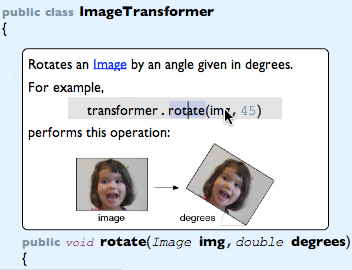
\includegraphics[width=.7\linewidth]{images/barista}
  \caption{A media-rich annotation in the Barista editor}
  \label{fig:barista}
\end{subfigure}%
\begin{subfigure}{.5\textwidth}
  \centering
  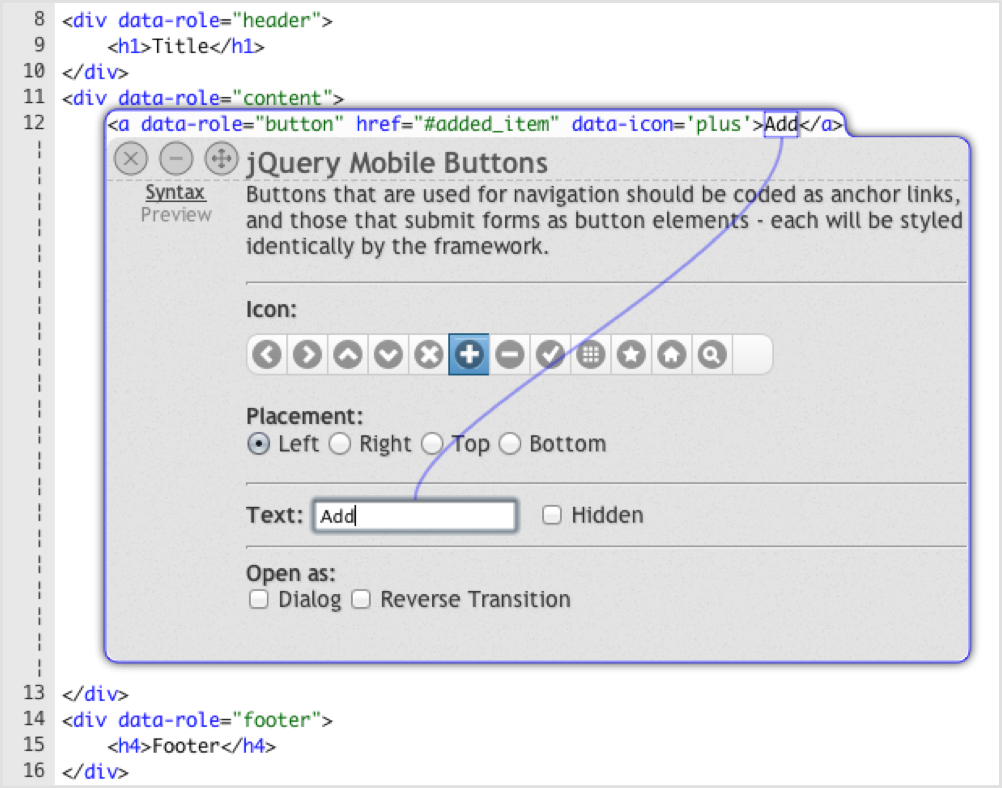
\includegraphics[width=.7\linewidth]{images/codelet}
  \caption{A Codelet inline helper}
  \label{fig:codelet}
\end{subfigure}
\caption{Example of media-rich annotations supported by code editors. On the left is Barista editor showing a Java method with richer annotations including images. On the right is the Codelets implementation showing the inline helper with icons defined for mobile buttons.}
\label{fig:richmedia}
\end{figure}

Barista~(Figure~\ref{fig:barista}) proposes a framework for creating interactive tools. It is build on top of Citrus~\citep{ko2005citrus}, a programming language intentionally created for supporting the creation of structured editors, it is consequently a positive factor that facilitates the implementation of new programming tools. These tools implement several principles of usability and readability, for example media-rich annotation of methods (including hyperlink and diagrams inside the comments; allowing show/dismiss the comments by double clicking), readable pretty-printed view of formulas (enabling edit of these expressions by double clicking), and so on. However, Barista seams to be more a prove of concept, than actually a system in use nowadays, besides the programming language used in this implementation be probably obsolete. On the other hand, Codelets~(Figure~\ref{fig:codelet}) uses media-rich resources to present in a pop-up a variety of icons that develops can choose to create their web pages. However, it is more related with code completion technologies than actually support program documentation.

The lack of tools that properly document a program is still a problem that negatively affects the \gls{gd} area. There is no such a tool which properly documents a program or automates the process of documentation. However, the support for implementing this kind of tool, and many other potentially useful, are poor or even inexistent in the majority of \gls{gd} systems. For example, in DesignScript~\citep{aish2012designscript}, Monkey, and many other textual environments, the source code is visually represented as rows of plain text, which makes difficult or even impossible the inclusion of rich-media elements (e.g. see Figure~\ref{fig:barista}). In the other hand, the visual programming languages, supported by environments such as Grasshopper and Dynamo, represent the source code visually with boxes and lines. However, to document these visual programming languages usually a box of plain text are provided, so that users can place it any where. As a result, the documentation becomes spread in a bunch of boxes randomly placed around the program, which makes difficult find out any useful information.

This problem is aggravated by the increasing use of \gls{gd} methods to support the design and conception of real architectural projects. The architectural projects, in the likeness of software projects, has a design phase where architects study the problem which they want to solve, analyze eventual constraints imposed by the client or external factors, and then define a draft of the solution. At the end of this process several artifacts are produced, such as diagrams and handmade sketches (as those portrayed in Figure~\ref{fig:sketch-fig}). These sketches are commonly used among architects since early days of architecture~\citep{do2001thinking}, because they represent a compact medium to convey complex ideas. The information generated in the design phase can be sufficient enough to model and construct the entire project serving as a start point, and a basis, to the development of the project. 

The Figure~\ref{fig:sketch-using} shows the importance of this phase in the architectural conception. In this example the architect started by drawing a series of  sketches annotating them with dimensional and spacial parameters such as height ($h$), diameter ($d$), the normal vector ($\vec{N}$), and vertex points (e.g. $P_0, P_1, P_2, ...$) of each shape (see Figure~\ref{fig:sketch-fig}). Then, he used those shapes, as a small piece of design, combining them to create a distinct pattern. After, he used this pattern applying it into a 2D sinusoidal surface which represents the ceiling of a geometric structure, as shown in Figure~\ref{fig:sketch-fig-result}. In this example is also clear the known approach in software engineering: \textit{dive to conquer}, because the architect started by designing the small pieces of the model and then he combined those unities of design to project his final structure. Understand this process is a fundamental step for proposing any useful programming tool.

\begin{figure}[h]
\centering
\begin{subfigure}{.6\textwidth}
  \centering
  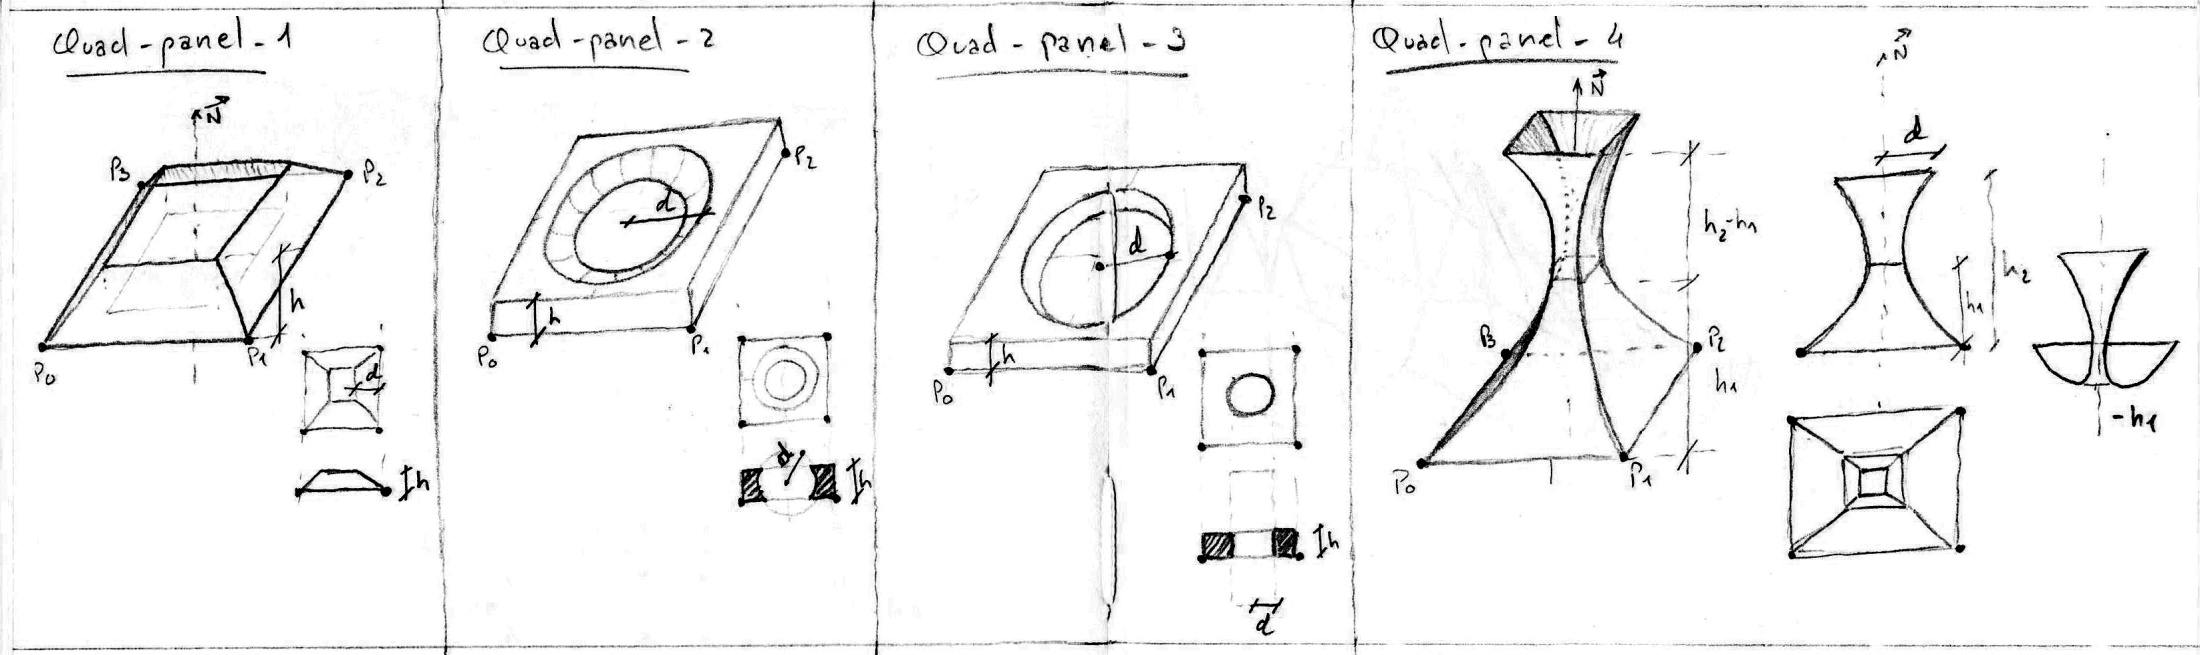
\includegraphics[width=.95\linewidth]{images/real-sketch}
  \caption{Sketches made during architectural design phase}
  \label{fig:sketch-fig}
\end{subfigure}%
\begin{subfigure}{.4\textwidth}
  \centering
  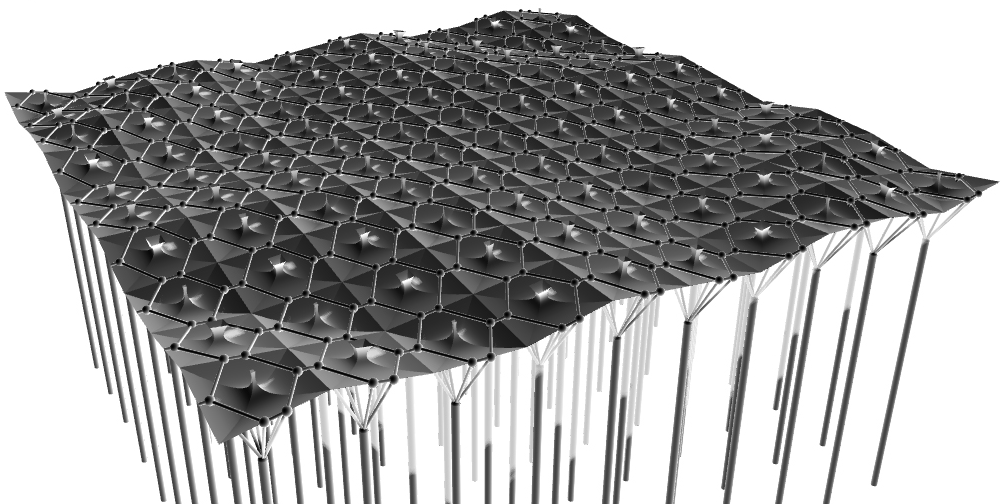
\includegraphics[width=1.0\linewidth]{images/real-sketch-result1}
  \caption{An application of the objects modeled previously in an architectural model}
  \label{fig:sketch-fig-result}
\end{subfigure}
\caption{Typical example showing the importance of design phase in the geometric model conception.}
\label{fig:sketch-using}
\end{figure}

In the context of \gls{gd} methods these sketches becomes even more relevant because they serve as basis for implementing the program. By definition of \gls{gd} method it formally defines a description of an architectural model~\citep{mccormack2004generative}. In this way, while the code defines the geometric object textually, the sketch define the geometric object visually. Consequently, it is fundamental during the development of the program but it is also a rich source for documenting the program. Different from the typical programs in software engineering which is purely textual and may express concepts that is difficult or even impossible to represent graphically, the program in \gls{gd} has this particularity of being able to represent its concepts through sketches or diagrams.

Surely sketches and diagrams are a suitable medium to express complex ideas. More than that, the architect frequently uses sketches because it helps him to reason about the conception of the design itself. And the \gls{gd} approach does not change this fact, on the contrary the use of sketch to illustrate program's components become even more popular, because it turns programming into a more  concrete and noticeable task, giving special clues for novice programmers. At the end of writing the program, all architect's decisions and insightful design, applied to construct the final program, are encapsulated in these sketches. As a result, these
sketches are also an essential artifact to comprehend the program specially after its release. 

For example consider the Figure~\ref{fig:chairseat} (reference here) that portrays a real example of a chair seat which was parametrically modeled. Even the less curious reader will wonder to know what each symbol of this image means. Some of them are more obvious than others, for instance the angles and the differences between them, however this diagram has its meaning embedded in problem context. It means that, those symbols in the image are variables which were created purposely to solve the problem of creating different shape of seats by varying the variable values. So the sketch proposes a parametric model of chair seats, additionally it contextualizes the meaning of each variable. Using this example the architect is able to create a suitable \gls{gd} method that creates this chair seat, however the \gls{gd} approach is not so straightforward as it seems to be. 

\begin{figure}[!htbp]
%\vspace{-5pt}
  \centering
  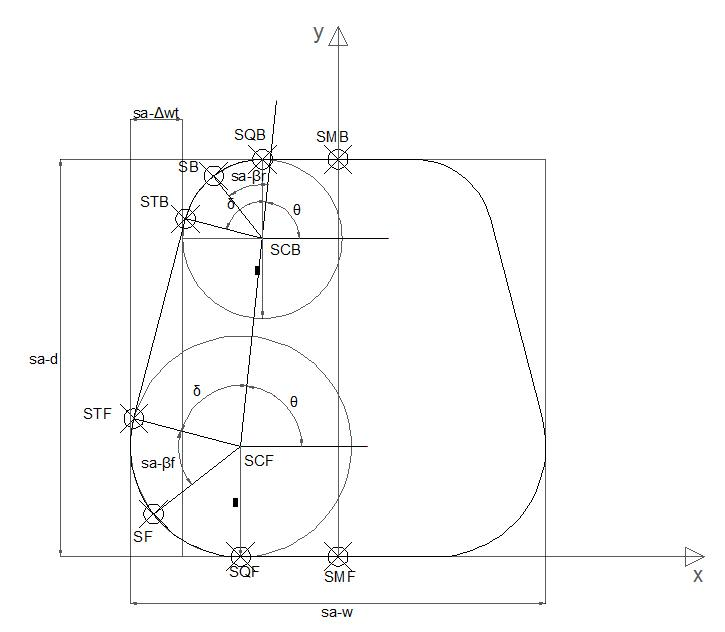
\includegraphics[width=0.5\textwidth]{images/seat}
    %\vspace{-15pt}
    \caption{A real sketch of a chair seat. In this sketch the seat is parametrized with some geometric variables. Some of them are intuitively noticeable, e.g. the angle symbols $\delta$, $\theta$, and $\beta$, but rest of them are not, because they have its meaning embedded in the problem context.}
    %\vspace{-5pt}  
  \label{fig:chairseat}
\end{figure}

The problem with the \gls{gd} methods is that when a geometric model is translated in a programming language all visual information that perhaps its diagrams show is lost. Therefore, we can not assume that architects has the same background of a software engineer, which means that they are expect to understand their models visually instead of interpreting symbols. So, the sketches are a rich source of information to guide the architect to comprehend the code, however when he look at the procedure that creates the model he will see instead something like the following code, shown in Listing~\ref{lst:chairseat}. \\ [3mm]

\begin{lstlisting}[
language=Python,
basicstyle=\ttm,
numbers=left,
stepnumber=1,
numbersep=5pt,                   
numberstyle=\scriptsize, 
caption={Sample of Python code that creates a chair},
label={lst:chairseat},
captionpos=b, 
otherkeywords={self},       % Add keywords here
keywordstyle=\ttb\color{deepblue},
emph={make_seat,__init__},       % Custom highlighting
emphstyle=\ttb\color{deepred},    % Custom highlighting style
stringstyle=\color{deepgreen},
frame=tb,                         % Any extra options here
showstringspaces=false            % 
]
def make_seat(smf, scf, scb, sa_d, sa_w, sa_deltawt, sa_betar, sa_betaf) :
   "this function creates a chair seat"
    ... # the seat logic
    return seat;
\end{lstlisting}

For the architect who did the sketch and implemented the code this function may appear simple enough to be understood. For people who will get this code posteriorly this kind of functions could be imperceptible nonetheless. Actually, in the architect's mind all these functions parameters make sense, because they are all part of the design (indeed the sketch can prove this). However, in most cases the sketches are not delivered with the program, even worst the program is usually delivered without any documentation or may have useless comments as that one in the example. Consequently, it negatively affects people who need to use this program, because without documentation they cannot understand the program well enough to use, or modify it, affecting the entire \gls{gd} community. 

\section{Sketch-program correlation tool}
\label{section:sc-tool}

As discussed in the previous section, the lack of documentation in \gls{gd} programs affects negatively its users. In fact this problem is beyond \gls{gd} area, it affects also the field of software engineering. In this field, there were attempts to improve this problem by improving the quality of program documentation, most prominently, \textit{literate programming}~\citep{knuth1984literate}. This work proposed a programming paradigm that promoted the fact that program are written for people first and foremost, and that documentation should be emphasized just as much as code. Unfortunately, these attempts did not reach the intended goals, mainly because writing good documentation takes considerable amount of time and effort.

A more recent work~\citep{learnableProg} suggested that the programming environment should minimize this tough work, required to write documentation, by automatically providing the documentation that programmers need when they are reading the code. In this work, Victor outlines the following idea:

\blockquote{The environment is responsible for making meaning transparent. The environment must enable the reader to effortlessly read the program, to decode the code, so he can concentrate on genuine programming concepts~\citep{learnableProg}}

Figure~\ref{fig:victor-ex} shows a prototype, presented with this work, that demonstrates how the environment can improve in the program readability. The code, on the left, is written in Processing language~\citep{Reas2006}, it sets the environment color to green and creates two geometric objects, on the right, a circle and rectangle, using the Processing functions: \texttt{fill, ellipse and rect}. This programming environment make the meaning of each element of code transparent, providing labels on mouse-over. For example, the reader will know that the fourth parameter of function \texttt{rect} will change the height of the rectangle, when he points to that parameter. And he can also point to every element of this code to get its meaning, so even before he makes any change in this code he will know exactly what the code is doing.     

\begin{figure}[!h]
%\vspace{-5pt}
  \centering
  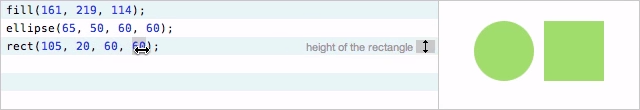
\includegraphics[width=.7\textwidth]{images/victor-example}
    %\vspace{-15pt}
    \caption{A programming environment that helps in the program readability. On the right, is a sample of code, written in Processing language, that creates a green circle and rectangle. On the right, is the produced result of this code. Each element of this program, including the functions and its arguments, are labeled so when user point the mouse over an element its label appears on the editor.}
    %\vspace{-5pt}  
  \label{fig:victor-ex}
\end{figure}

Labeling the program elements on mouse-over indeed make the program meaning more explicit, but this technique does not replace the need of a proper documentation. The main problem with this approach is that these labeled functions already exist in Processing, so this feature is more intended to avoid unnecessary searches on the Processing manual, than alternatively provides a way to document the program. For any user defined function this feature will not work, consequently the programmer must take considerable amount of time and effort to create its own documentation.

The reality in architecture is quite different form that in software engineering: it is part of the design process to produce documentation in the form of sketches. This means that it is not necessary to write huge amounts of textual documentation to explain a \gls{gd} program. We only need to annotate the already existing sketches and combine them with the program, thus providing visual explanations of what the program is supposed to do.

In Figure~\ref{fig:sc-tool} I propose the \textit{sketch-program correlation tool} that shows how sketches and code can be combined to provide useful documentation for the programmer by using the sketches made in a early phase of program design. This example illustrates a function that draws an arrow giving the base point $P$, the direction $\alpha$, the height $\rho$, and the width $\beta$ and size $\sigma$ of the arrow tip. This information is all condensed in the sketch, maybe even more precise. So the idea of this tools is to take advantage of this fact by pointing out what is the meaning of each function parameter, found in the code, in the context of the sketch (and vice versa). In this way, when the user has the mouse over a function parameter he immediately sees what that parameter correspond in the sketch, and  the inverse is also valid: when he moves the mouse over a symbol in the image he immediately see its meaning in the code. That helps him to create a mental model of the program even before to change it.

\begin{figure}[!htbp]
%\vspace{-5pt}
  \centering
  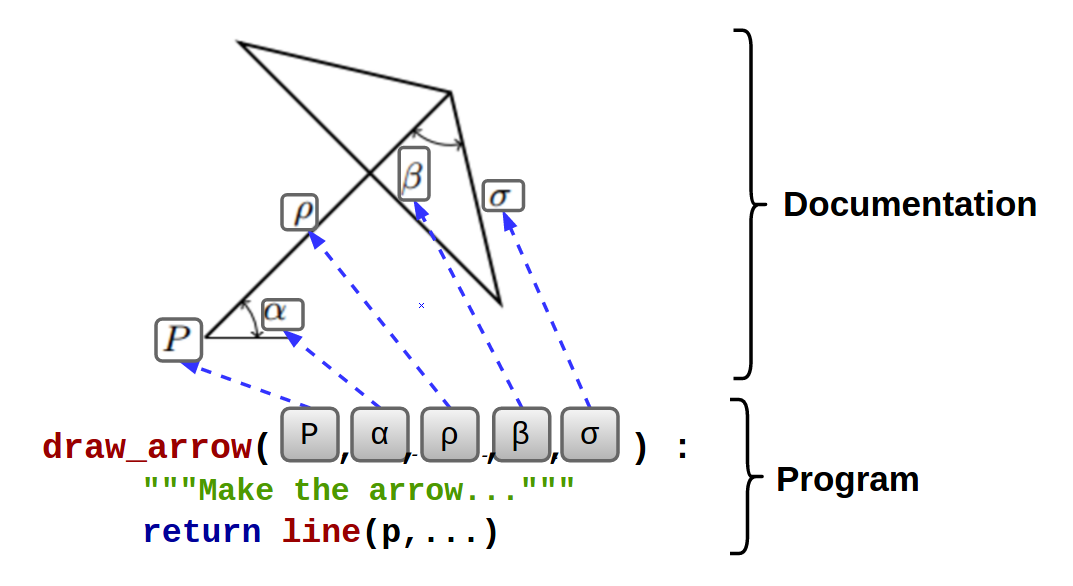
\includegraphics[width=0.5\textwidth]{images/proposed-sc-tool}
    %\vspace{-15pt}
    \caption{\textit{Sketch-program correlation tool} showing how to combine fragments of the program with sketches. In this example all the function parameters has a correspondent symbol in the sketch that illustrate its meaning}
    %\vspace{-5pt}  
  \label{fig:sc-tool}
\end{figure}

As demonstrated in early works, the underline principle behind this tool can in fact helps in the program readability, consequently helping in the overall process of program comprehensibility. However implement this tool in the current environments for \gls{gd} is undoubtedly a hard  challenge, due the absence of certain capabilities required for implementing this kind of tool considering the current state of \gls{gd} environments.

Perhaps the first challenge imposed by this tool, is in how to include images in the code editor. It seems a trivial problem, however the possibility to insert a simple image in the code editor is unsupportable for at least the majority of code editors. Specially in \gls{gd} where the environments used for textual languages generally only support rows of plain text. Until the time we are not aware of any other code editors that provide such a capability, in exception of Rosetta tool~\citep{lopes2011portable} that provides an enhanced code editor that supports images and other media-rich elements, by using DrRacket~\citep{findler2002drscheme} as its code editor.

A inherent concern in the fact of supporting images in the code editor is on how to store it. The strategy used by DrRacket, is to serialize the image and store it in ascii-encoded binary format. The problem of this strategy is that once the programmer inserts an image in his code and save it, he will not be able to change its code again using other text editor. So this method does not provide any backwards-compatibility with other text editors potentially useful to write programs. As a result, it makes difficult, or even impossible, the portability of the program among those different text editors.

I propose another approach to this problem that assures backwards-compatability. The first step is to define a standard annotation that will be used to include the image, similarly to the Java doc annotation. Then requires the use of that annotation upon an event of image insertion. Thus to include an image the programmer should quote the image with that annotation, as the example depicted in Figure~\ref{fig:inline-image}. As a result, it will be possible for the program environment to distinguish images from source code and proceed to an adequate treatment for those images. 

\begin{figure}[!htbp]
%\vspace{-5pt}
  \centering
  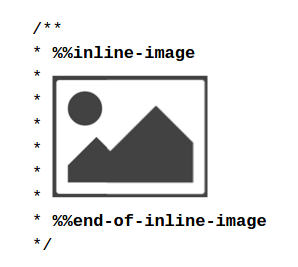
\includegraphics[width=.25\textwidth]{images/inline-image-example}
    %\vspace{-15pt}
    \caption{Example of inline-image annotation.}
    %\vspace{-5pt}  
  \label{fig:inline-image}
\end{figure}

By using this convention, when the programmer save his code all images under that annotation can be stored as a simple source code comment. For example considering that source code comment which includes an image showed in Figure~\ref{fig:inline-image}. If the programmer open that code in an editor that does not support this annotation the following string will be showed instead:

\begin{center}
\begin{minipage}[c]{.6\textwidth}
\texttt{// \%\%image \$\{USER\_HOME\}/project/sketch1.jpg \%\%}
\end{minipage} \\
\end{center}

The above text is a convection that represents a relative path from where the code editor loaded the image. In this way if the code editor cannot resolve this path and find the image, the code could be showed anyway by displaying just that comment, thus the code can be opened in any text editor. Of course to be able to see the images, programmers must open the code in the text editor capable to interpret that annotations and display the images. 

Other systems, to avoid the problem of incompatibility among editors convert the code into a textual format, for example Barista~\citep{ko2006barista} saves the code in XML. However the presented approach goes further, because it does not impose any language specific requirement, the code is stored as it is (ordinary plain text). So it is up to the code editor to implement suitable methods to show the images.

Nevertheless, an interesting challenge imposed by the sketch-program correlation tool is the automatic recognition of text and symbols in images. Fortunately, this is an old problem which is part of the ancient dream of replicating the human functions by machines, making the machine able to perform tasks like reading. To concertize this dream was realized that information should be readable both to humans and to machine and alternative inputs can not be predefined. As consequence of this probably inputs, an \gls{ocr} system would be necessary for dealing with the problem of recognizing optically processed characters. Optical recognition is performed after the writing or printing has been completed. Therefore the idea of this system is avoiding the traditional way of entering data into a computer through the keyboard by providing a more efficient way for it.

The \gls{ocr} systems rapidly became a prominent field of study that gave substantial incentives for making pattern recognition and image analysis matured fields of science. The very first attempts can actually be found back in 1870~\citep{eikvil1993optical} with the retina scanner which was an image transmission system using a mosaic of photocells. From then, consecutive attempts were made to improve the methods of \gls{ocr} systems, specially by sophisticating the retina scanner and creating OCR machines that became commercially available in the 1950's. Posteriorly, HP as a possible software and/or hardware add-on for HP's line of flatbed scanners, proposed a novel open-source project: Tesseract~\citep{smith2007overview} OCR engine. This project was then sponsored by Google and nowadays is one of the most accurate OCR engine on the market used widely in several web applications.

Clearly the subject of character recognition is extremely extensive and its details are beyond the scope of this dissertation. However, to propose my solution of recognizing automatically text in image, I based on the functioning of the \gls{ocr} engine, namely the Tesseract~\citep{smith2007overview}, that accepts an image file and returns a file with the recognized characters and their respective coordinates. However, the Tesseract is a local application that needs to be installed in the user's computer, or be included as an external library, which may affect the portability of the application and its use.

To overcome this problem I propose the use of \gls{ocr} Web Services, such as OnlineOCR\footnote{\texttt{http://www.onlineocr.net/}}, or FreeOCR\footnote{\texttt{http://www.free-ocr.com/}}. These engines provide the same functionality as Tesseract, most of them are build on top of it, but provide a standard way for integrating it in the application by using protocols such as SOAP, or REST. Figure~\ref{fig:sc-tool-arch} shows the proposed architecture for this tool, where their components are described as following:

\begin{itemize}
\item \textit{Code Editor.} Is the programmer \gls{ui} where images and code will be inserted. So this component is the first filter of the pipe, consequently it starts the logic sequence flow of processing the image.
\item \textit{Image Filter.} This component has two main activities: first get the image inserted on the editor, and second send the image to the OCR Engine through REST invocation. (Note: it assumes that the web service provides a suitable service for this, which is naturally usual among the \gls{ocr} Web Services studied.)
\item \textit{OCR Engine.} Is the fundamental piece of this architecture, where the image will be processed and transformed in optical characters. This component is a kind of bottle-neck because the correct operation of this tool depends on how well this engine will operate. As accurate the character recognition be as well the tool will work.
\item \textit{Meta-data Collector.} This component is intended to receive the information processed by the \gls{ocr} engine and then store it. This information contains the optical characters that were successfully recognizes by the engine and additionally the image coordinate from where each symbol was picked. 
\end{itemize}

\begin{figure}[!htbp]
%\vspace{-5pt}
  \centering
  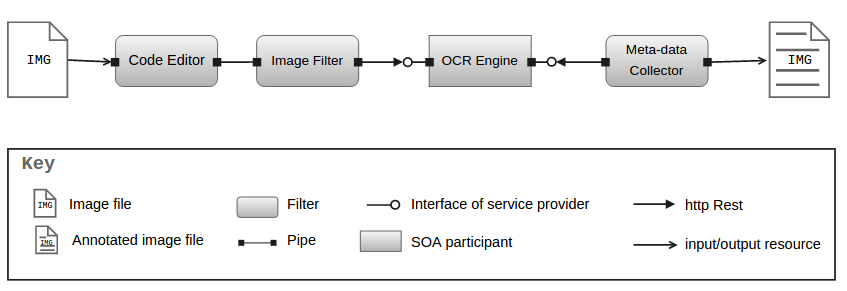
\includegraphics[width=.7\textwidth]{images/sc-tool-architecture}
    %\vspace{-15pt}
    \caption{Data flow view combining two styles: pipe-and-filter style and client-server style.}
    %\vspace{-5pt}  
  \label{fig:sc-tool-arch}
\end{figure}

The presented architecture left several open questions, for example an evident issue is where the information generated by the \gls{ocr} engine will be stored. This decision is hard to make immediately, because it is intrinsically related with the way which the programming environment stores its rich-media elements. As discussed earlier, there are several approaches to it, such as serialize the elements as binary format, convert the code to textual information using standard formats i.e. XML, and, the presented approach, use conventional source code comments to wrap the rich-information. The strategy used for storing meta-data with the image may vary depending on the output format chosen. What I propose is to use the last option: wrapping with the image its characters an respective coordinates due its apparent advantage relatively to the other approaches.

The \gls{ocr} engine uses a pattern recognition that is pretty susceptible to errors. In this case I propose a fallback mechanism that delegates the task of recognizing symbols to the programmer. Thus the programmer can directly intervene in the image recognition process by helping the \gls{ocr} upon a mistake. It is a rich source of information for the \gls{ocr} as well, because this data can be used as a corpus of training, thus improving  in the capabilities of the engine. After of processing the image and get its characters, the next step is to meaningfully present this information to the programmer.

In this point we have the code and the plain text extracted from the image, then the problem is how to combine them with code. I propose two alternatives to overcome this problem as follows:

\begin{enumerate}
\item \textit{Implement a programming environment from scratch.} This option allow a high level of customization, because the environment can be built base on this requirement. Thus adequate technologies can be chosen purposely to deal with images in code and eventually support the binding between code and image graphically, as shows Figure~\ref{fig:sc-tool} for instance. Moreover, the tool is language independent, it only requires the image meta-data to be able to connect symbols in the image with code characters. This approach can also minimize the effort to add other features, because different tools share the same core implementation. Despite of the apparent advantages, there is a huge effort to implement a new environment and of course a risk of this environment not be used by the target users. For example Barista~\citep{ko2006barista} takes this approach by providing an environment for Java programmers, however it is very unlikely that a Java programmer will use this tool in his daily tasks.

\item \textit{Extending an existing programming environment.} It is a straightforward approach based on the fact that most programming environments nowadays provide some kind of support for add-on features. In this way, programmers can create new features without changing the programming environment itself by implementing a common \gls{api}. The main advantage of this approach is that we can use  resources generated by other tools without having to implement them, e.g. the \gls{ast}, a rich resource, generated in the compiling phase, is usually provided through \glspl{api}. Moreover, the programming language can be used to achieve this goal, some programming languages allow the definition of new grammar rules, consequently a new grammar rule can be created in order to consider images as part of grammar. However this approach is extremely dependent of the language/environment support for add-ons and, consequently, the \gls{api} provided by the existing system.
\end{enumerate}

Finally an important issue that affects the entire system is related with the usability of the programming environment. Adding images mixed with code is something that can impair the usability of the programming environment, because it can occupy a considerable part of the editor making the program readability difficult. Moreover when programmers are coding, they are concentrating on that task and the images may be a kind of distraction. So, this is a common sense problem that does not have a straight solution, conversely I propose some strategies to avoid this problem:

\begin{itemize}
\item Treat image and rich-media resources as text. It means that programmers should be able to work with rich-media resources such as working with text character, so it can be cut and paste, it can be deleted, it can be moved by dragging and drop, and also it can be indented, just like text.

\item Support text caret navigation as it is in text editor. Evidence from a study of programmers' low-level text editing strategies~\citep{ko2005design} suggests that programmers rely heavily on the keyboard for code navigation. Therefore, adding rich-media resources in the source code can interfere in the caret navigation. However, treating images as text will not affect the caret navigation.

\item Show or dismiss the rich-media resources by double clicking. The purpose of this facility is to avoid any kind of distractions, so when the programmer is coding he can simply double click on the image to dismiss it and concentrates in the code editing.

\item Add images by dragging and drop, and support inline edition. It is important for the user that add images, or other resources, be fairly simple as write code. Mechanism like dragging and drop must be provided, as well as facilities to edit the image directly in the editor, or alternatively open it in a system editor, and save it. As 
fewer iterations are needed to edit an image as better will be for the programmer.
\end{itemize}


\section{Immediate feedback tool}

Programming is an unobservable task that is mainly performed in programmer's head. As discussed in Chapter~\ref{chapter:background}, programming is hard to learn, because it involves knowledge about the subject, strategies to apply this knowledge, and fundamentally it requires that the programmers maintain many different kinds of ‘mental model’ which is the way they comprehend their programs~\citep{robins2003learning}. However work in our mind is something that does not scale, and blindly manipulate symbols is not truly programming.

There were several attempts for making programming a more tangible task. For example, the ancient technique of debugger tools is precisely to enable programmers to see the state of their programs, its structures, and the flow of information that pass through it upon execution. With successive improvements of these tools, recent systems, such as LightTable~\citep{lighttable}, have been tried to anticipate as much as possible the result of a program change. That means, this environment reduces the delay between an edition in the source code and its visualization. This is a simple concept in practice, but it becomes popular in the academic community and even beyond them in the industry context. For example, JRebel is a popular tool that allows developers to visualize their changes in a web application without to stop the application server. So, visualize changes allow programmers to test their mental models consequently improve their comprehension about the program.

While programmers work in their minds, architects by contrast work in their sketches~\citep{do2001thinking}. In fact sketches are a suitable media for drafts, and even better for experimenting and testing new ideas and visualize them quickly, which is the fundamental key for creating novel designs. However the \gls{gd} methods change drastically this reality, instead of interacting directly with the model, as traditionally in Architecture, the architect interacts with a model's intermediate: i.e. the program that specifies it. Thus, any change in the model must be performed firstly in the code and then only after the execution of the program the architect will be able to see the impact of his change in the model. This process delays the visualization of the model, consequently it affects negatively the design conception.

Notable efforts have been made in \gls{gd} area to overcome this limitation. For example, the visual programming languages, such as Grasshopper, Dynamo, among others, provide immediate feedback. Which means that as the user interacts with the language components, by adding and connecting them, the result reflects immediately in the \gls{cad} tool. However as the visual programs become large and complex it requires more time to understand, maintain, and adapt to new requirements, than the textual programs~\citep{leitao2011programming}. On the other hand, the programming environments that support textual language usually do not support immediate feedback at all.

To overcome this limitation, I propose an immediate feedback tool aimed for textual programming languages. The goal of this tool is to reduce substantially the time between a change in the code and its effect in the program execution. Thus, architects will be able to change their programs and instantaneously see the impact of that change in the geometric model. As a result, it allows program experimentation, and eventually it will improve the program comprehension. Moreover, this tool provide a foundation for other features which can be implement on top of it.

However to improve the program experimentation is first necessary to find out which are the activities of this process and where programmers spend the most of time. Consider the chair seat model shown in Figure~\ref{fig:chairseat}, assuming that this model was already implemented and the architect needs to use it to generate some samples of seats. The activities of this process is shown in Figure~\ref{fig:run-activity}, and they are described as follows:

\begin{itemize}
\item Find places to change in the source code. The time spent to perform this step may vary substantially, because it depends on the complexity of the program, and on the architect's knowledge about the program. Unfortunately these factors are not directly related with this tool, instead it is more related with the tool presented in Section~\ref{section:sc-tool}.

\item Edit the source code, that means choose the right parameters with suitable values to perform the desired change. Precious time is spent in this step, because usually the architect needs to predict the range of values that makes sense for a certain parameter. Fortunately, this step can be improved by this tools and the time can be spared.

\item Run the program. Depending on the programming environment this step can be performed by a simple click on a button, until execute a command to compile and run the program. In fact, this step can be optimized using appropriate techniques, for example reuse previous computation.

\item Visualize the change in the model, and check if the code change was sufficient to generate the desired model, otherwise repeat the process. This is one of the most time consuming activity, because it relies on \gls{cad} tool to generate the model. As discussed previously, \gls{cad} tools are not designed to process the huge amount of information generated by \gls{gd} methods, consequently to optimize this activity alternative backends must be consider.   
\end{itemize}

\begin{figure}[!htbp]
  \centering
  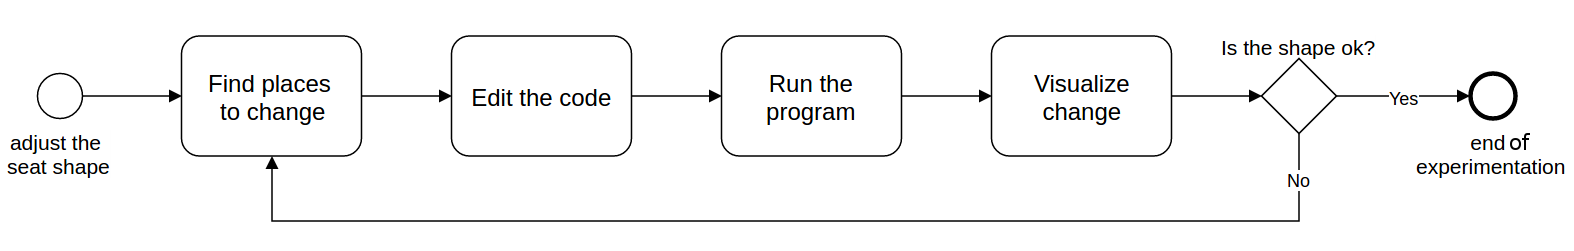
\includegraphics[width=1\textwidth]{images/run-activity}
    \caption{Activity diagram for adjusting the shape of the chair}
  \label{fig:run-activity}
\end{figure}

Base on those activities, a reasonable approach to implement the immediate feedback feature is to optimize the program execution. Some programming systems, such as Impromptu~\citep{sorensen2005impromptu}, and Fluxus \citep{griffiths2007fluxus}, attempt to address this with a so-called "live coding" environment, where the output updates immediately as the code changes. These system use a common technique to provide this feature: a language interpreter that given an expression immediately evaluates it. Curiously, both of live coding systems referred use the Scheme interpreter (a Racket~\citep{findler2002drscheme} interpreter ascendant) due its enhanced capabilities. For example, the Scheme runtime can be integrated with other programming languages like C, and C++, the interpreter already provides a sandbox mechanism, consequently it only executes code syntacticly correct avoiding compilation errors, among others facilities. However in these programming systems any change in the code will cause the entire program to be interpreted.

An apparent improvement in performance is related with the utilization of previous computation that was unchanged after a code edit. Consider the following sample of code that creates a chair given a point, its height and width, and the seat dimensions. \\ 

\begin{lstlisting}[
language=Python,
basicstyle=\ttm,
numbers=left,
stepnumber=1,
numbersep=5pt,                   
numberstyle=\scriptsize, 
caption={Sample of Python code that creates a chair},
label={lst:offset},
captionpos=b, 
otherkeywords={self},       % Add keywords here
keywordstyle=\ttb\color{deepblue},
emph={make_chair,__init__},       % Custom highlighting
emphstyle=\ttb\color{deepred},    % Custom highlighting style
stringstyle=\color{deepgreen},
frame=tb,                         % Any extra options here
showstringspaces=false            % 
]
offset = 50
def make_chair(p_center, ca_h, ca_w, sa_d, sa_w) :
   real_p = xyz(p_center.x/offset, p_center.y/offset, p_center.z/offset)
   # some complex computation
   chair = create_chair_obj(ca_d, ca_w, sa_d, sa_w)
   return move_to(real_p, chair)
# creates a chair in origin
make_chair(xyz(0, 0, 0), 20, 20, 30, 30)
\end{lstlisting}

Supposing that the function \pythoninline{create_chair_obj} does the major part of computation by calculating the points and creating the chair object, and the \pythoninline{move_to} function only translate the model to that given point. If the architect moves the chair position (e.g. change it to $\{ x\!=\!1,y\!=\!1,z\!=\!1 \}$) it seems unnecessary recalculate the entire chair, because it was already calculated and this change does not affect the shape of the model. As a result of reusing this computation the operation will be a simple translation, however this solution will not work in some cases. For example, the global variable \pythoninline{offset} is a constant for the program, and a common optimization of the compiler, called constant folding, is to replace every occurrence of that variable by its value. The resultant program would look like this: \\

\begin{lstlisting}[
language=Python,
basicstyle=\ttm,
numbers=left,
stepnumber=1,
numbersep=5pt,                   
numberstyle=\scriptsize, 
caption={Sample of Python code that creates a chair after constant folding},
label={lst:offset-change},
captionpos=b, 
otherkeywords={self},       % Add keywords here
keywordstyle=\ttb\color{deepblue},
emph={make_chair,__init__},       % Custom highlighting
emphstyle=\ttb\color{deepred},    % Custom highlighting style
stringstyle=\color{deepgreen},
frame=tb,                         % Any extra options here
showstringspaces=false            % 
]
offset = 100
def make_chair(p_center, ca_h, ca_w, sa_d, sa_w) :
   real_p = xyz(p_center.x/50, p_center.y/50, p_center.z/50)
   # some complex computation
   chair = create_chair_obj(ca_d, ca_w, sa_d, sa_w)
   return move_to(real_p, chair)
# create a chair in origin
make_chair(xyz(1, 1, 1), 20, 20, 30, 30)
\end{lstlisting}

The problem happens if the architect decides to change the offset parameter, this alteration will not have impact in the model. Because the \pythoninline{make_chair} is reusing a computation which the offset was 50, and besides it was changed the model will not reflect it because it needs to be compiled again. This technique may result by allowing the user only change function parameters, but such restriction can turn this tool useless. Other technique are used for example, the design script implements a data flow language that in this case a change in the offset would e propagated through its decencies. On the other hand YinYang reuses previous computation by allowing only the changed graphs in the \gls{ast} be compiled. However these languages were tailored specifically for this purpose, and is outside the scope of this thesis create a better mechanism that the first approach.

An relevant issue associated with the textual languages in \gls{gd} is the lack of mechanisms that facilitate the program experimentation. Each time the architect wants to change a geometric model, he needs to blindly edit the code, guessing an appropriate input. This is an ineffective way to edit the program, besides of being a laborious process for experimentally generating new models, it clearly discourages all the creative work which is fundamental in the design conception.

On the other hand, the visual programming languages, such as Grasshopper and Dynamo, understand this as a serious limitation in architectural work. They provide some interesting mechanisms to avoid it, such as interactive widgets which facilitate the process of program experimentation. For example, in Grasshopper users can add a widget, also known as slider, in a component input that allows a program variable be defined in a range of values, then the user can test each of those values by simply dragging the mouse over the range  (as shown in Figure~\ref{fig:grass}).

Similar technique, by contrast, is used in live-code environments like Fluxus~\citep{griffiths2007fluxus} and Impromptu~\citep{sorensen2005impromptu}. Although these programming systems are associated to textual programming languages, they provide sliders to allow performers to quickly change their programs input. For example, the function in Figure~\ref{fig:sc-tool} will generate the \gls{ui} portrayed in Figure~\ref{fig:slider-ui}.  

\begin{figure}[!htbp]
  \centering
  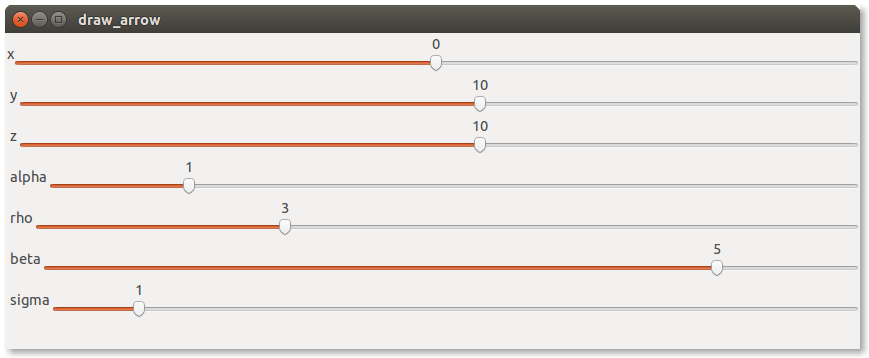
\includegraphics[width=0.6\textwidth]{images/slider-sample}
    \caption{A slider user interface for the draw-arrow function.}
  \label{fig:slider-ui}
\end{figure}

The problem with this \gls{ui} is that nothing is labeled, to understand the meaning of each slider's parameter programmers must find out in the documentation or spend time studying the code. Likewise, this \gls{ui} is exactly as informative as this line of code:

{\centering
  \pythoninline{draw_arrow(xyz(0, 10, 10), 1, 3, 5, 1)}\par
}

Clearly, the code is more acceptable than the \gls{ui}, the information is exactly the same but it is presented in a condensed way. That helps the programmer to get more information about the context from where that function is called. Moreover he can interact directly with the code, rather than be distracted by the \gls{ui}. However, there is no facilities to edit program values interactively, as in slider widget for instance.

To overcome this limitation, I propose a slider mechanism that facilitates the change of each program literal. Instead of showing a \gls{ui} with all function parameters at once (as shown in Figure~\ref{fig:slider-ui}), this mechanism allows each function parameter be changed individually, creating a unique slider on top of that parameter. As a result, programmers can interactively change the program input without being overwhelmed by a \gls{ui} which contains more information than the programmer needs. Moreover, this mechanism is independent of the program execution, that means dragging the slider will only edit the code. Obviously to have any immediate  effect in the program execution, the program should be re-executed at any slider drag.

Unfortunately, immediate feedback will not scale with the increasing complexity of \gls{gd} programs. When the programmer drags the slider, he is expecting to see how that alteration looks like in the model. Likewise, when we are writing in a text editor, we are expecting to see how the words look like, otherwise we will probably think that something is going wrong. Show the hidden states of the program is an important heuristic, specially in this context where users are depending on the program result. However, implement this heuristic in the current \gls{gd} environments would be a hard challenge.

Grasshopper is a concrete example of system that has faced this problem insistently. The first approach of Grasshopper was change the model at any change in the slider. In this way, as the program becomes complex as long its execution takes, reaching at a certain point which the programmer becomes afraid to touch in the slider so that the program does not freeze. The second approach was to restrict the slider input to only accept textual inputs. Of course, this approach was severely criticized by the users because it was against the principles of visual programming languages. Rapidly a new strategy was proposed: deactivate the effect of slider dragging only reproducing the final dropped value. This strategy has a better performance, however the architect is expecting to find out a set of values that creates a novel design, using this method he only be able to experiment individual values instead of a range of values at once.

There is a straight solution for this problem, as discussed above, which is the use of an alternative backend. For this tool, I propose to use an alternative backend working as a kind of playground where users can create samples, and find out the right parameters to build their models. Base on the fact that a program in \gls{gd} produces the similar result independently of the backend chosen, consequently the parameter values found in the experimental phase can be used by simply change the backend. Moreover sliders can be used to interactively create new models.

However sliders must have helpful values that makes sense for that program input. For example in Figure~\ref{fig:slider-ui}, the parameters showed have a distinct range of values, i.e. $\{x,y,z\} \in \mathds{R}$ and the angles $\{\alpha,\beta, \sigma, \rho \} \in [0, 2 \pi]$. The problem is how to predict the correct range of values given a function parameter. In principle the program variables declared as integer have their domain in $\mathds{R}$, so the challenge is to restrict this domain to something that makes sense for that particular invocation. There are several strategies used in practice, for instance LightTalbe~\citep{lighttable} shows a drop down list where the first value is a minor value (i.e. $x \in \mathds{R}^- : x \rightarrow - \infty$) and the last value is a major value (i.e. $x \in \mathds{R}^+ : x \rightarrow + \infty$) and depending on the chosen value the next drop down list will be shown a range of values closer to the previous one.

Based on  live-code environments, I propose a clever alternative which is to initially show a reduced range of values ($x \in \mathds{R} : x \in [x-10, x+10]$) and then adapt this range of values accordingly to the user experimentation. That means, initially the range is statically defined and the increment between the values is also constant. As quicker the programmer drags the slider as greater will be the increment between the values, consequently changing the range of values. As a result architects will be able to experiment different range of values in their programs by simply dragging the slider.

However the possibility of dragging the slider through a range of values can be error prone. For example consider the Snippet of code~\ref{lst:offset}, if the programmer decides to vary the values of \pythoninline{offset} an error will occur when it reaches to zero, because there are some division using this value. In this situation there are two alternatives to follow: (1) stop the experimentation and present the error, or (2) omit the error and allow the programmer to continue in his task. I propose the second alternative once the goal of this tool is to allow program experimentation, in this way a proper sandbox mechanism must be implemented.

To conclude, in this chapter I presented some problems associated with programming in general. Then, I focused in \gls{gd} area which is a popular area specially among novice programmers. However, the current \gls{gd} environments are not designed to introduce the basics of good software engineering practice, such as document the program, or even support user interactions such as connecting the architects to their designs. To overcome those limitation I proposed general ideas, and then a proposed solution of two interactive tools: sketch-program correlation, and immediate feedback. In the next chapter I present an evaluation of these ideas.